\documentclass[aspectratio=169]{beamer}
\usepackage[utf8]{inputenc}
\usepackage[T1]{fontenc}
\usepackage[brazil]{babel}
\usepackage{lmodern}
\usepackage{braket}
\usepackage{bookmark}
\usepackage{listings}
\usepackage{xcolor} % Necessário para usar cores
\usepackage{verbatim} % Necessário para usar cores
\usepackage{hyperref} % Essencial para URLs clicáveis e seguras


% --- USE O TEMA QUANTUM ---
\usetheme{Quantum}

% \lstset{
%   backgroundcolor=\color{lightgray!20},   % Cor de fundo
%   basicstyle=\ttfamily\small,            % Estilo da fonte (monospaçada e pequena)
%   commentstyle=\color{green!60!black},    % Cor dos comentários
%   keywordstyle=\color{blue},             % Cor das palavras-chave
%   numberstyle=\tiny\color{gray},         % Estilo dos números de linha
%   stringstyle=\color{purple},            % Cor das strings
%   breaklines=true,                       % Quebrar linhas longas
%   breakatwhitespace=true,                % Quebrar linhas apenas em espaços
%   captionpos=b,                          % Posição da legenda (b=bottom)
%   keepspaces=true,                       % Manter espaços no código
%   numbers=left,                          % Onde colocar os números de linha (left, right, none)
%   numbersep=5pt,                         % Distância dos números até o código
%   showspaces=false,                      % Não mostrar espaços
%   showstringspaces=false,                % Não mostrar espaços dentro de strings
%   showtabs=false,                        % Não mostrar tabs
%   tabsize=2                              % Tamanho da tabulação
% }

% \hypersetup{
%     colorlinks=true,
%     linkcolor=blue,
%     filecolor=magenta,      
%     urlcolor=blue, % Deixa as URLs azuis e clicáveis
%     pdftitle={Referências},
% }

% --- INFORMAÇÕES DA APRESENTAÇÃO ---
\title{Otimização de funções em módulo 2 utilizando DQI}
\subtitle{Algoritmo DQI max-XORSAT}
\author{Daniel Nocito \and Diogo Vieira \and Rafael Campos}
\institute{UFRJ}
\date{02 de Julho de 2025}

\begin{document}

% --- PÁGINA DE TÍTULO ---
\begin{frame}
  \titlepage
\end{frame}

% --- SLIDE DE ROTEIRO ---
\begin{frame}
  \frametitle{Roteiro}
  \tableofcontents
\end{frame}

\section{Entendimento do Problema}
\begin{frame}
  \frametitle{O Problema max-XORSAT}

  O é max-XORSAT? Traduzindo, significa :
  \begin{center}
    \textit{Maximizar a Satisfabilidade do XOR.}
  \end{center}

  Ou seja, encontrar um string binário (ou vetor) que satisfaça o maior número possível de equações lineares em $\mod 2$.

\end{frame}

% --- SLIDE DEFINIÇÃO DA FUNÇÃO OBJETIVO ---
\section{Definição da Função Objetivo}
\begin{frame}
  \frametitle{Definição da Função Objetivo}
  \begin{itemize}
    \item Como maximizar o número de equações satisfeitas?
  \end{itemize}
  Ora, um sistema linear em módulo 2 é da forma:
  \[
  Ax=b \mod2
  \longleftrightarrow
    \begin{cases} 
      a_{11} x_1 + a_{12} x_2 + \cdots + a_{1n}x_n = b_1 & \text{(mod 2)} \\
      a_{21} x_1 + a_{22} x_2 + \cdots + a_{2n}x_n = b_2 & \text{(mod 2)} \\
      \vdots \\
      a_{m1} x_1 + a_{m2} x_2 + \cdots + a_{mn}x_n = b_m & \text{(mod 2)}
    \end{cases}
    \]
  
  Para a função objetivo, definimos o resultado intermediário para cada linha como
  $$
  \begin{cases}
    1, & \text{se } a_i\cdot x = b_i \\
    -1, & \text{se } a_i\cdot x \neq b_i \\
  \end{cases}
  $$
\end{frame}

\begin{frame}
  \frametitle{Definição da Função Objetivo}
  Voltando ao problema max-XORSAT, a função objetivo $f(x)$ é, então, o somatório dos resultados intemediários:
  \[
    f(x)=\sum_{i=1}^m (-1)^{a_i \cdot x + b_i}
  \]

  \vfill
  \begin{block}{Ideia Geral da Func. Objetivo}
    Essa função objetivo conta o número de equações cuja escolha de $x$ satisfaz e subtrai o número de equações que não satisfazem.
  \end{block}
\end{frame}

% --- SLIDE DEFINIÇÃO DO PROBLEMA ---
\section{Definição do Problema}
\begin{frame}
  \frametitle{Definição do Problema}
    \textbf{Entrada:} Um sistema linear na forma de:
    \begin{itemize}
      \item Uma matriz $A \in \mathbb{F}_2^{m \times n}$; e
      \item Um vetor $b \in \mathbb{F}_2^m$ com $m > n$.
    \end{itemize}
    \vfill
    \textbf{Saída:} Um vetor $x \in \mathbb{F}_2^n$ que melhor maximiza $f$, definida adiante.
  \vfill
  \begin{block}{O Problema max-XORSAT}
  \begin{itemize} 
    \item \textbf{Objetivo:} Encontrar x que melhor soluciona a equação $Ax=b \mod2$.
    \item \textbf{Metodologia}
    \begin{itemize}
        \item Definir uma função objetivo $f(x)$.
        \item Aplicar o Algoritmo de Interferometria Quântica Decodificada (DQI).
    \end{itemize}
  \end{itemize}
  \end{block}
\end{frame}

\subsection{Por que usar o DQI?}
\begin{frame}
  \frametitle{Por que usar o DQI?}
  O problema Max-XORSAT é classificado como \textbf{NP-difícil}!

  \vfill
  \begin{block}{Vantagens do DQI}
    \begin{itemize}
      \item O DQI foca em encontrar soluções \textit{aproximadas}.
      \item A estratégia é reduzir um problema de otimização a um problema de decodificação usando a \textit{Transformada de Fourier Quântica (QFT)}.
    \end{itemize}
  \end{block}
\end{frame}


\section{Algoritmo DQI}
% --- SLIDE ALGORITMO DQI ---
\begin{frame}
    \frametitle{Algoritmo DQI}

    \textbf{Passos do Algoritmo de Intereformetria Quântica Decodificada (DQI):}
    \vfill

    \begin{enumerate}
        \item Preparação do Estado Inicial
            \begin{itemize}
                \item Criação de Superposição Uniforme
            \end{itemize}
        \vfill
        \item Codificação da Função Objetivo na Fase (Oráculo)
            \begin{itemize}
                \item Aplicar efeito da Função Objetivo
            \end{itemize}
        \vfill
        \item Aplicação da Transformada Quântica de Fourier (QFT)
            \begin{itemize}
                \item Causa interferência construtiva para favorecer as soluções desejadas
            \end{itemize}
        \vfill
        \item Medição e Decodificação Clássica
            \begin{itemize}
                \item Leitura da Superposição e interpretação clássica
            \end{itemize}
    \end{enumerate}
\end{frame}

\subsection{Circuito do DQI}
\begin{frame}
  \frametitle{Algoritmo DQI}

  \textbf{Circuito Quântico:}

  \vspace{1cm}

  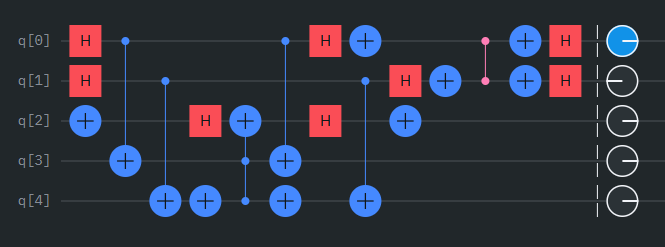
\includegraphics[scale=0.5]{circuito.png}
  % \begin{figure}
    
  % \end{figure}
\end{frame}

% --- SLIDE PREPARAÇÃO DO ESTADO INICIAL ---
\subsection{Preparação do Estado Inicial}

\begin{frame}[fragile]
  \frametitle{Preparação do Estado Inicial}

  Criação de estado de \textbf{Superposição Uniforme} de todos os $2^n$ estados possíveis para o vetor $x$ de variáveis.
  Isso é feito aplicando Hadamard em todos os registros.

  \vfill

  \begin{block}{Resultado da 1ª Etapa}
  Aplicando Hadamard a $n$ qubits no estado $\ket{0}$, resulta em:
  \[
    \ket{\psi_0}=\frac{1}{2^n} \sum_{x\in\{0,1\}^n}\ket{x}
  \]
  \end{block}

  \begin{block}{Implementação no Simulador Python \lstinline|cirq|}
  \begin{lstlisting}[language=Python, frame=single, basicstyle=\tiny]
def preparar_estado_inicial(qubits):
    return cirq.Circuit(cirq.H.on_each(qubits))
  \end{lstlisting}
  \end{block}

\end{frame}

% --- SLIDE CODIFICAÇÂO DA FUNÇÃO OBJETIVO NA FASE ---
\subsection{Codificação da Função Objetivo na Fase}

\begin{frame}
  Nessa etapa, a função objetivo é incorporada na \textit{fase} estado quântico. 

  \vfill

  Isso é feito através de um polinômio $P(f(x))$ da função objetivo, em que $P(f(x))\ket{x}$ é proporcional a amplitude do estado.

  \frametitle{Codificação da Função Objetivo na Fase}
  \[
      \ket{\psi_P}=N \sum_{x\in\{0,1\}^n}P(f(x))\ket{x}
  \]
  \begin{block}{Transformação com o Polinômio Objetivo}
      \begin{itemize}
          \item $N$ é a constante de normalização; e
          \item $P(f(x))$ é o polinômio da função objetivo.
      \end{itemize}
  \end{block}
\end{frame}

\begin{frame}[fragile]
  
  \begin{block}{Implementação no Simulador Python \lstinline|cirq|}
  \begin{lstlisting}[language=Python, frame=single, basicstyle=\tiny]
def create_phase_oracle(x_qubits, B_mat, v_vec):
    n_vars = len(x_qubits)
    m_eqs = len(v_vec)
    y_qubits = [cirq.NamedQubit(f'y_{i}') for i in range(m_eqs)]
    phase_qubit = cirq.NamedQubit('phase_ancilla')
    
    compute_Bx = [cirq.CNOT(x_qubits[j], y_qubits[i]) for i in range(m_eqs) for j in range(n_vars) \
                                                                                    if B_mat[i, j] == 1]
    flip_to_target = [cirq.X(q) for i, q in enumerate(y_qubits) if v_vec[i] == 0]
    apply_phase = [
        cirq.X(phase_qubit), cirq.H(phase_qubit),
        cirq.X(phase_qubit).controlled_by(*y_qubits),
        cirq.H(phase_qubit), cirq.X(phase_qubit)
    ]
    return cirq.Circuit(compute_Bx, flip_to_target, apply_phase, list(reversed(flip_to_target)), \
                                                                             list(reversed(compute_Bx)))
  \end{lstlisting}
  \end{block}
\end{frame}

\subsection{Tranformada Quântica de Fourier}
\begin{frame}
  \frametitle{Tranformada Quântica de Fourier}

  Nessa etapa, aplicamos a QFT em $|\psi_P\rangle$. 
  \vfill
  \textit{Fisicamente}, a QFT causa uma interferência construtiva nas amplitudes dos estados que correspondem às características importantes da função objetivo. 
  Nossa função objetivo possui seu espectro de Fourier \textbf{esparso} (i.e., a informação está concentrada em poucos coeficientes de Fourier: $N$ ou $-N$).
  
  \begin{block}{Relembrando a QFT}
    A QFT de $n$-qubits atua em um estado da base $|\mathbf{x}\rangle$ da seguinte forma:
    $$
    \text{QFT}|\mathbf{x}\rangle = \frac{1}{\sqrt{2^n}} \sum_{\mathbf{y} \in \{0,1\}^n} (-1)^{\mathbf{x} \cdot \mathbf{y}} |\mathbf{y}\rangle
    $$
  \end{block}
\end{frame}

\begin{frame}[fragile]
  
  \begin{block}{Implementação no Simulador Python \lstinline|cirq|}
  \begin{lstlisting}[language=Python, frame=single, basicstyle=\tiny]
def create_diffusion_operator(x_qubits):
    circuit = cirq.Circuit()
    circuit.append(cirq.H.on_each(x_qubits))
    circuit.append(cirq.X.on_each(x_qubits))
    if len(x_qubits) > 1:
      circuit.append(cirq.Z(x_qubits[-1]).controlled_by(*x_qubits[:-1]))
    elif len(x_qubits) == 1:
      circuit.append(cirq.Z(x_qubits[0]))
    circuit.append(cirq.X.on_each(x_qubits))
    circuit.append(cirq.H.on_each(x_qubits))
    return circuit
  \end{lstlisting}
  \end{block}
\end{frame}

\subsection{Medição}
\begin{frame}
  \frametitle{Medição}

  Após a aplicação da QFT, é aplicada a \textbf{medição}! 

    \vspace{1cm}
  
  A medição é a etapa na qual é realizada a leitura dos qubits e interpretado para sua identificação do vetor $x$ desejado 

\end{frame}

\section{DQI em Ação}
\begin{frame}
  \frametitle{DQI em Ação}

  Hora do vídeo!
  
\end{frame}

\section{Considerações Finais}
\begin{frame}
  \frametitle{Considerações Finais}
  
  \begin{itemize}
    \item O DQI acha uma boa aproximação para um problema que é originalmente NP-Difícil!
    \item Ele é direcionado a problemas como o max-XORSAT com matrizes $A$ esparsas, que se reduzem a problemas de decodificação.
    \item Em uma instância de exemplo com 31.216 variáveis e 50.000 restrições, o DQI alcançou 83,5\% de restrições satisfeitas, enquanto o simulated annealing (heurística) obteve 81,5\%. Outras heurísticas como o algoritmo AdvRand (55,4\%) também foram superadas.
    \item Caso de uso bastante restrito!
  \end{itemize}
  
\end{frame}

\section{Referências Bibliográficas}

\begin{frame}[fragile]
  \frametitle{Referências Bibliográficas}
  
  \begin{enumerate}
    \footnotesize
    \item BARTSCHI, A.; EIDENBENZ, S.. Deterministic Preparation of Dicke States. \textit{arXiv (Cornell University)}, 15 ago. 2024.
    \item CLASSIQ TECHNOLOGIES. \textit{Decoded Quantum Interferometry Algorithm - Classiq}. Disponível em: \url{https://docs.classiq.io/latest/explore/algorithms/dqi/dqi_max_xorsat/}. Acesso em: 29 jun. 2025.
    \item HARI. Linear Block Codes: Encoding and Syndrome Decoding. \textit{MIT - Lecture Notes}. Disponível em \url{https://web.mit.edu/6.02/www/s2012/handouts/6.pdf}. Acesso em: 29 jun. 2025.
    \item JORDAN, S. \textit{Quantum Algorithm Zoo}. Disponível em: \url{https://quantumalgorithmzoo.org/#JSW24}. Acesso em: 29 jun. 2025.
    \item JORDAN, S. P. et al. Optimization by Decoded Quantum Interferometry. \textit{arXiv (Cornell University)}, 15 ago. 2024.
    \item SCHMIDHUBER, A. et al. Quartic quantum speedups for planted inference. \textit{arXiv (Cornell University)}, 27 jun. 2024.
    \item YAMAKAWA, T.; ZHANDRY, M. Verifiable Quantum Advantage without Structure. \textit{arXiv (Cornell University)}, 5 abr. 2022.
  \end{enumerate}
  
\end{frame}

\end{document}